\part{Metodologia}
\chapter[Metodologia]{Metodologia}

Tendo como meta a definição de um modelo de ML para ser aplicada em uma RNA a ser treinada para detecção de intrusão, a estratégia a ser seguida é o fluxo de trabalho de aprendizado de máquinas, descrito na figura 6 (\ref{fig06}).

\section{Construção do Modelo}
    No processo básico de \textit{feature engineering} exitem alguns passos a serem tomados.

    \begin{itemize}
        \item Pré-processamento dos dados: \\ Neste primeiro passo, é montado o modelo de dados de treinamento que será usado para apresentação e utilização dos dados. Para isso é necessário encontrar uma corelação entre os dados de entrada e o dado a ser atingido pelo processo de aprendizado. A partir do momento que a corelação é encontrada, os dados devem ser dispostos de modo que facilite sua visualização e uso, sendo assim de acordo com \cite{brink2015}, é recomendado que se convertam os dados categóricos (normamente textuais) em dados numéricos, para facilitar seu uso.
        \item Treinamento do modelo: \\ O modelo proposto deve passar por um breve treinamento utilizando-se de algorítmos de ML que verificam a aplicabilidade do modelo de dados para se construir um modelo de ML. Estes algorítmos utilizam os chamados \textit{tuning parameters}, que são os parâmetros utilizados pelo algorítmo durante a leitura dos dados e são utilizados para definir o quão complexa é a relação entre os dados de entrada e o valor alvo. \cite{brink2015}
        \item Avaliar o modelo: \\ Uma vez com o modelo pronto é necessário avaliar a aplicabilidade do modelo em vista dos dados que se querem atingir. Um exemplo simples de avaliação é a comparação dos dados que deveriam ter sido atingidos com os dados preditos pelo modelo, como exemplifica a tabela a seguir:
        \newpage

        \begin{table}[]
            \centering
            \caption{Class-wise accuracy}
            \label{accuracy-table}
            \resizebox{0.65\textwidth}{!}{%
            \begin{tabular}{|l|l|l|ll}
                \cline{1-3}
                Test set Labels & Value equals             & Predictions &  &  \\ \cline{1-3}
                1               &  True                    & 1           &  &  \\ \cline{1-3}
                0               &  True                    & 0           &  &  \\ \cline{1-3}
                1               &  True                    & 1           &  &  \\ \cline{1-3}
                1               &  False                   & 0           &  &  \\ \cline{1-3}
            \end{tabular}}
        \end{table}

        Esta tabela simplificada mostra uma forma fácil e rápida de calcular se o modelo está gerando os resultados esperados. Neste caso, com 3 acertos em 4 valores tem-se 75\% de acerto. \cite{brink2015}

        \item Escolher as \textit{features}: \\ Neste momento as \textit{features} que deverão ser utilizadas dentro do modelo de ML são selecionadas.
    \end{itemize}

    \subsection{Como escolher as features}
        Existem várias formas diferentes de se escolher um bom conjunto de \textit{features}, aqui serão listados os dois algorítmos mais difundidos:
        \begin{itemize}
            \item Algorítmo \textit{Forwards Selection}: \\ Consiste em aplicar um algorítmo no conjunto total de \textit{features} que vai testar uma por uma selecionando para um novo grupo de \textit{features} que serão utilizadas somente as que possuem maior eficácia na avaliação de predição de valores.

            \begin{figure}[ht]
                \centering
                \label{fig06}
                    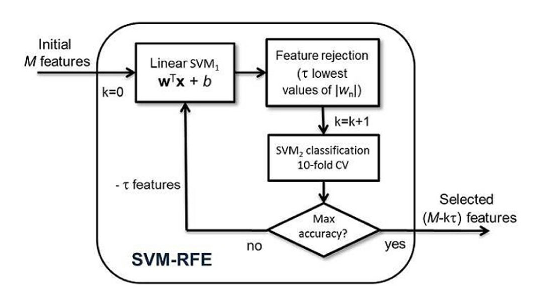
\includegraphics[keepaspectratio=true, scale=1.2]{editaveis/images/forward-selection.eps}
                \caption{Representação do ciclo de \textit{Forward-selection}.}
                Fonte : \url{http://goo.gl/270zF3}
            \end{figure}

            \item Algorítmo \textit{Backwards Elimination}: \\ Consiste em aplicar um algorítmo no conjunto total de \textit{features} que vai testar uma por uma selecionando para um novo grupo de \textit{features} que serão eliminadas somente as que possuem menor eficácia na avaliação de predição de valores.

            \begin{figure}[ht]
                \centering
                \label{fig06}
                    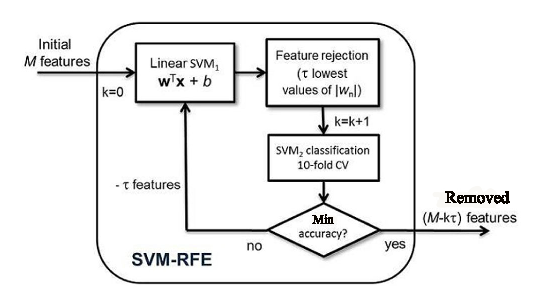
\includegraphics[keepaspectratio=true, scale=1.2]{editaveis/images/backward-selection.eps}
                \caption{Representação do ciclo de \textit{Backward-selection}.}
                Fonte : \url{http://goo.gl/270zF3}
            \end{figure}

        \end{itemize}

        Segundo \cite{brink2015}, estes algorítmos não garantem o melhor conjunto de features possível, porém eles entregam um conjunto aproximado das melhores features encontradas em cada iteração.

